%  Autor: Ismael Felipe Ferreira dos Santos
%         Instituto de Fisica,
%         Universidade Federal de Alagoas
%  E-mail: ismaellxd@gmail.com
%  Copyright © 2019 MIT LICENCE
%  Turorial LaTeX: https://ismaeldamiao.blogspot.com/p/latex.html
%  Descrição: Modelo de documento feiro em LaTex, o foco principal do modelo é 
%            fazer o relatório de trabalho/experimento, entretanto este modelo
%            pode ser seguido para quaisquer outros fins que necessitem do LaTeX
\documentclass[
   % -- opções da classe memoir --
   12pt,                         % tamanho da fonte.
   openright,                    % capítulos começam em pág ímpar (insere página vazia caso preciso).
   oneside,                      % para impressão em recto. Oposto a toweside.
   a4paper,                      % tamanho do papel. 
   sumario = tradicional,        % Para indentar os sumários
   % -- opções da classe abntex2 --
   chapter=TITLE,                % títulos de capítulos convertidos em letras maiúsculas.
   section=TITLE,                % títulos de seções convertidos em letras maiúsculas.
   subsection=TITLE,             % títulos de subseções convertidos em letras maiúsculas.
   subsubsection=TITLE,          % títulos de subsubseções convertidos em letras maiúsculas.
   % -- opções do pacote babel --
   english,                      % idioma adicional para hifenização.
   french,                       % idioma adicional para hifenização.
   spanish,                      % idioma adicional para hifenização.
   brazil,                       % O último idioma é o principal do documento.
   xcolor=table                  % Tabelas coloridadas.
]{abntex2}
% --------------------------------------
% PACOTES
% --------------------------------------
% Nesta parte estão os pacotes importados, cada pacote adciona uma função nova
\usepackage[cleanup]{gnuplottex}       % Para uso do GNUPlotTex.
\usepackage{graphicx}                  % Inclusão de gráficos.
\usepackage{chemfig}                   % Para notação química.
\usepackage[version=3]{mhchem}         % Para notação química.
\usepackage{amssymb}                   % Para exibir símbolos de conjuntos de números (reais, etc...).
\usepackage{amsmath}                   % Para adcionar equações
\usepackage{amsfonts}                  % Fontes para notação matemática.
\usepackage{amsthm}                    % Para adcionar Teoremas
\usepackage{thmtools}                  % Front end para amsthm (\declaretheorem)
\usepackage[T1]{fontenc}               % Selecao de codigos de fonte.
\usepackage[utf8x]{inputenc}           % Codificacao do documento (conversão automática dos acentos).
\usepackage{ucs}                       % Complemento do anterior.
\usepackage{indentfirst}               % Indenta o primeiro parágrafo de cada seção.
\usepackage{float}                     % Para posicionar figuras corretamente.
\usepackage{subcaption}                % Para legendas nas subfiguras.
\usepackage[table,xcdraw]{xcolor}      % Para tabelas coloridas.
\usepackage{multirow}                  % Para mesclar  linhas nas tabelas.
\usepackage{color}                     % Controle das cores.
\usepackage{microtype}                 % para melhorias de justificação.
\usepackage{lipsum}                    % para geração de dummy text.
\usepackage{fancyhdr}                  % Pemite alterações no cabeçalho e rodapé.
\usepackage{hyperref}                  % Cria formatação automática de PDF.
\usepackage[hyphenbreaks]{breakurl}    % Quebra de linha em url.
\usepackage{geometry}                  % Permite configurar as margens da página.
\usepackage[num,overcite]{abntex2cite} % Citações padrão ABNT, em ordem alfabética.
\citebrackets[]                        % Citações com coxetes.
\usepackage{setspace}                  % Espaço duplo entre parágrafos.
% --------------------------------------
% CONFIGURAÇÕES DE PACOTES
% --------------------------------------
% Não se impote com essas coisas, no geral, não será preciso mexer nelas
\renewcommand{\ABNTEXchapterfontsize}{\Large}       %Muda o tamanho da fonte de título de capítulo
\renewcommand{\ABNTEXchapterfont}{\rmfamily}        %Muda a fonte do título de capítulo
\renewcommand{\ABNTEXsectionfontsize}{\large}       %Muda o tamanho da fonte de título de seção
\renewcommand{\cftchapterfont}{\rmfamily}
\renewcommand{\cftchapterpagefont}{\normalsize\cftchapterfont}
\renewcommand{\cftsectionfont}{\rmfamily}
\renewcommand{\cftsectionpagefont}{\cftsectionfont}
\setlength\afterchapskip{\lineskip}


% Aqui as páginas estão ajustadas segundo as regras da ABNT
\geometry{hmargin={3cm,2cm},vmargin={3cm,2cm}}          %Mudar margens da página

% Tem aguma coisa a ver com a química, sem isso o pacote parece não funcionar
% direito
\newcommand\setpolymerdelim[2]{\def\delimleft{#1}\def\delimright{#2}}
\def\makebraces[#1,#2]#3#4#5{%
\edef\delimhalfdim{\the\dimexpr(#1+#2)/2}%
\edef\delimvshift{\the\dimexpr(#1-#2)/2}%
\chemmove{%
\node[at=(#4),yshift=(\delimvshift)]
{$\left\delimleft\vrule height\delimhalfdim depth\delimhalfdim
width0pt\right.$};%
\node[at=(#5),yshift=(\delimvshift)]
{$\left.\vrule height\delimhalfdim depth\delimhalfdim
width0pt\right\delimright_{\rlap{$\scriptstyle#3$}}$};}}
\setpolymerdelim()

% Aqui eu utilizei o pacote de teoremas para criar também a funções para axiomas
% leis físicas, e definições matemáticas
\declaretheorem[style=definition,name=Definição,parent=chapter,qed=\textemdash]{definicao}
\declaretheorem[style=plain,name=Teorema,qed=\textnormal{\textemdash}]{teorema}
\declaretheorem[style=plain,name=Axioma,qed=\textnormal{\textemdash}]{axioma}
\declaretheorem[style=plain,name=Lei,qed=\textnormal{\textemdash}]{lei}

% --------------------------------------
% CONFIGURAÇÕES DA CAPA
% --------------------------------------
% Em geral, nessas configurações você só precisara mudar as imagens no 
% \includegraphics e seus tamanhos
\renewcommand{\imprimircapa}{%
   \begin{capa}%

      \centering

      \begin{figure}

         $\vcenter{\hbox{
\includegraphics[width=1.0cm]{UFAL}}}$\hfill
            % Na pasta onde foi extraido este modelo tem uma imagem chamada
            % UFAL.png substitua essa imagem pela logo da sua universidade
         \begin{minipage}[c]{0.6\textwidth}
            \center
            \imprimirinstituicao
         \end{minipage}
         \hfill$\vcenter{\hbox{
\includegraphics[width=1.0cm]{IF}}}$
            % Na pasta onde foi extraido este modelo tem uma imagem chamada
            % IF.png substitua essa imagem pela logo do seus instituto

      \end{figure}

      \vspace*{1cm}

      \imprimirautor

      \vfill
      \imprimirtitulo
      \vfill

      \imprimirlocal \\
      \imprimirdata

   \end{capa}
}
\makeatletter
% --------------------------------------
% CONFIGURAÇÕES DA FOLHA DE ROSTO
% --------------------------------------
\renewcommand{\folhaderostocontent}{
   \centering

   \imprimirautor \\
   \vspace{5cm}
   \imprimirtitulo \\

   \vfill
   \begin{flushright}
      \begin{minipage}{.5\textwidth}
         \imprimirpreambulo
      \end{minipage}%
      \vspace{0.5cm}
      \begin{minipage}{.5\textwidth}
         Orientador \imprimirorientador
      \end{minipage}%
   \end{flushright}
   \vfill

   \imprimirlocal \\
   \imprimirdata
   \pagenumbering{arabic} %Começa a contar as páginas
}
\makeatother
% --------------------------------------
% Informações de dados para CAPA e FOLHA DE ROSTO
% --------------------------------------
% Nesta parte ainda não são permitidos ascentos, segue um dicionário
% cedilha ç = \c{c}
% cedilha Ç = \c{C}
% agudo á = \'{a}, Á = \'{A}
% agudo é = \'{e}, É = \'{E}
% agudo í = \'{i}, Í = \'{I}
% agudo ó = \'{o}, Ó = \'{O}
% agudo ú = \'{u}, Ú = \'{U}
\titulo{T\'{I}TULO DO TRABALHO \\ 
        RELAT\'{O}RIO DE AULA PR\'{A}TICA} % Não aceita ascento
\autor{NOME DO ALUNO} % Não aceita ascento
\local{Maceió} % Aceita ascento
\data{2020}
\orientador{Prof.º Dr. Fulano de tal} % Aceita ascento
\instituicao{UNIVERSIDADE FEDERAL DE ALAGOAS \\ 
             INSTITUTO DE F\'{I}SICA \\
             F\'{I}SICA - BACHARELADO} % Não aceita ascento
\tipotrabalho{Relatório de experimento} % Aceita ascento
\preambulo{Relatório do experimento 'título do trabalho' realizado no 
           laboratório de física 1, como requisito para avaliação da disciplina 
           Física Experimental 1.} % Aceita ascento

\begin{document}
% Aqui é onde comça o documento, todo comando colocado aqui modifica alguma 
% coisa no documento, voçê somente precisar fazer edições depois do início dos 
% elementos textuais
% ------------------------------------------------------------------------------
% ELEMENTOS PRÉ-TEXTUAIS
% ------------------------------------------------------------------------------

% ---
% CAPA & FOLHA DE ROSTO
% ---
   \imprimircapa
   \imprimirfolhaderosto
% ---
% SUMÁRIOS
% ---
   \clearpage
   \pagebreak % Quebra de página
   \listoffigures*
   \listoftables*
   \tableofcontents*
   \pagebreak
% ------------------------------------------------------------------------------
% ELEMENTOS TEXTUAIS
% ------------------------------------------------------------------------------
   \textual

   \chapter{Introdução} % Adciona um capítulo cujo título é informado ente {}
      \vspace{0.5cm}

      % Note que você pode começar a adcionar seus texto e usar ascentos
      % Considere que o texto não comentado também está te disendo algo
      A Introdução é onde é feito um resumo histórico e teórico sobre o que
      está sendo estudado.

      \ref{eq:nomedaequacao} O Comando prescedente faz uma citação ao que está 
      entre {} enquanto que o comando que se segue adcionada uma equação 
      numerada:

      \begin{equation}
         \label{eq:nomedaequacao} % Aqui é onde você dá um nome ao bloco, nesse
         % caso equação, para se referir a ele durante o texto com o \ref{}.
         \sum_{i=1}^{n} \vec F=\sum_{i=1}^{n} \frac{d\vec p}{dt}=\sum_{i=1}^{n} \ddot{\vec p}
      \end{equation}

      \noindent este comando serve para adcionar uma linha não indentada.

      Confira em \url{https://pt.wikipedia.org/wiki/Ajuda:Guia_de_edi%C3%A7%C3%A3o/F%C3%B3rmulas_TeX}
      um guia completo sobre os comandos para utilizar notação matemática em 
      $\LaTeX$.

      E sim $x=x_0cos(\omega_0t)$, dessa forma é possível adcionar equações 
      no meio de uma linha simplesmente colocando a equação entre $$.

      \begin{equation}
         \label{eq:part2}
         T=2\pi \sqrt{\frac{m}{k}}
      \end{equation}

      Os parágrafos da introdução precisam ter cidatas as fontes onde você 
      aprendeu o que está dizendo. Este comando server pra 
      isso.\cite{LoiElectricite}\cite{moyses1}
      
      Utilizei os seguintes comandos para enunciar a primeira lei do movimento 
      de Newton:
      
      \begin{lei}
         Corpus omne perseverare in statu suo quiescendi vel movendi uniformiter in directum, nisi quatenus illud a viribus impressis cogitur statum suum mutare.\cite{principia1}
      \end{lei}

      Essa é uma citação da segunda lei do movimento
      \footnote{Este comando server para adcionar uma nota de rodapé}
      \footnote{Sir Isaac Newton}:

      \begin{citacao}
         Lex II: Mutationes motis proportionalem esse vi motrici impressæ, et fieri secundum lineam retam qua vis illa imprimitur. - N. Isaac\cite{principia1}
      \end{citacao}
      
      Este comando serve para adcionar um teorema:
      
      \begin{teorema}
         Sejam $\varphi_j : \mathbb{R} \rightarrow \mathbb{R}, j = 1, ..., n$\: $n$ funções de classe $C^n$, se o Wronskiano 
         associado a estas funções é não-nulo então ela são linearmente independentes.
      \end{teorema}

      Aproveito os comando de axioma para enunciar os três pilares da lógica:

      \begin{axioma}Identidade\\
      Toda proposição é equivalente a si mesma.
      \end{axioma}

      \begin{axioma}Não contradição\\
      Toda proposição ou é falsa ou é verdadeira nunca os dois.
      \end{axioma}

      \begin{axioma}Identidade\\
      Toda proposição é exclusivamente ou falsa ou verdadeira nunca outro.
      \end{axioma}

      \section{Seção}

         Isto é uma Seção.

         \subsection{Sub-seção}

            Isto é uma Sub-seção.

            \subsubsection{Sub-sub-seção}

               Isto é uma Sub-sub-seção.

   {\let\clearpage\relax % para não quebrar página de um capítulo a outro
   \chapter{Objetivos}
      \vspace{0.5cm}}

      \begin{itemize}
         \item Verbos no infinitivo;
         \item Verificar a lei tal;
         \item Medir tal coisa.
      \end{itemize}

      {\let\clearpage\relax
   \chapter{Materiais utilizados}
      \vspace{0.5cm}}

      \begin{itemize}
         \item 1 objeto;
         \item n objetos.
      \end{itemize}

      {\let\clearpage\relax 
   \chapter{Procedimentos}
      \vspace{0.5cm}}

      Verbos no passado e em terceira pessoa.

      Foi feito isso, mediu-se aquilo.

      {\let\clearpage\relax 
   \chapter{Dados e análise}
      \vspace{0.5cm}}

      Mostre tabelas e gráficos com os dados.

      Organize esses dados de tal forma que eles informem algo, aqui os dados serão expostos de tal forma que mais adiante seja possível tirar conclusões deles.

      Com o \LaTeX  podemos adcionar tabelas:

      \begin{table}[H]
         \centering
         \caption{\label{tab:part1}\footnotesize Título}
         \begin{tabular}{c|cccc}
            Haste    & $t_1(s)$ & $t_2(s)$ & $t_3(s)$ & $t_4(s)$ \\ \hline
            Cobre    & 41       & 74       & 99       & 135      \\
            Alumínio & 35       & 57       & 89       & 129      \\
            Latão    & 56       & 107      & 181      & 239     
         \end{tabular}
      \end{table}

      \noindent confira \url{https://tablesgenerator.com/}.

      Com o \LaTeX  podemos adcionar figuras:

      \begin{figure}[H]
         \centering
         \caption{\label{fig:coordenadas}\footnotesize Título.}
         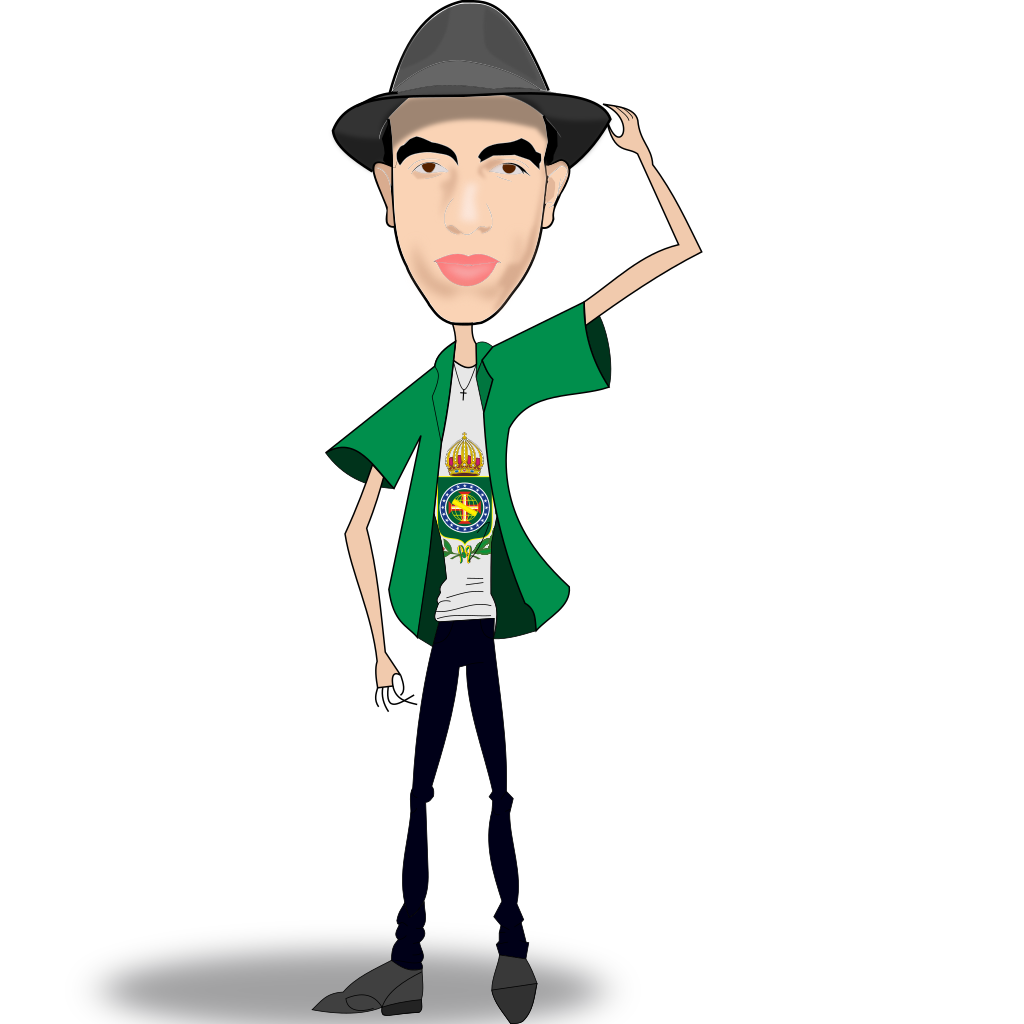
\includegraphics[scale=0.2]{img/NomeDoArquivo}
         \legend{\footnotesize Fonte:}
      \end{figure}

      \noindent ou

      \begin{figure}[H]
         \centering

         \begin{subfigure}[t]{0.4\textwidth}%
            \centering
            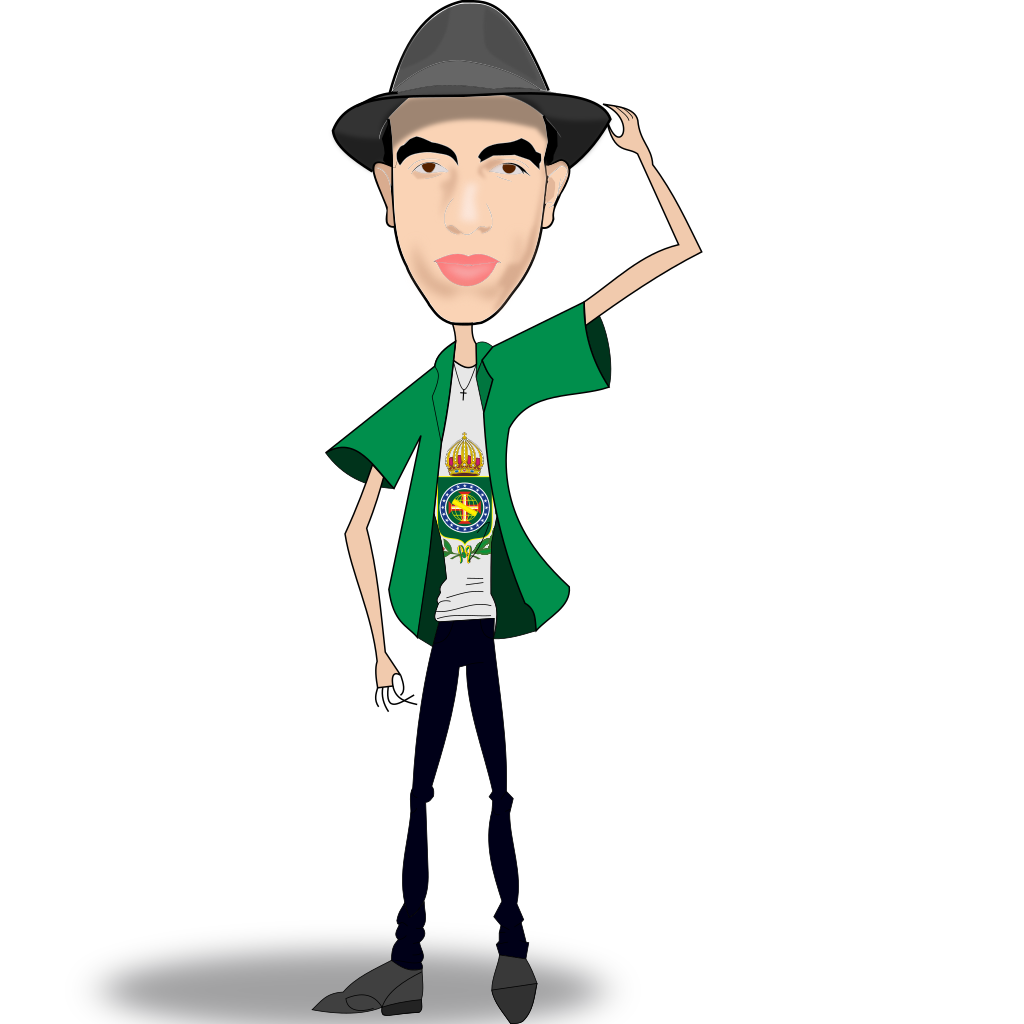
\includegraphics[scale=0.1]{img/NomeDoArquivo}
            \caption{\label{fig:placas}\footnotesize Exemplo de duas figuras.}
         \end{subfigure}
         \hspace{0.1cm}
         \begin{subfigure}[t]{0.4\textwidth}%
            \centering
            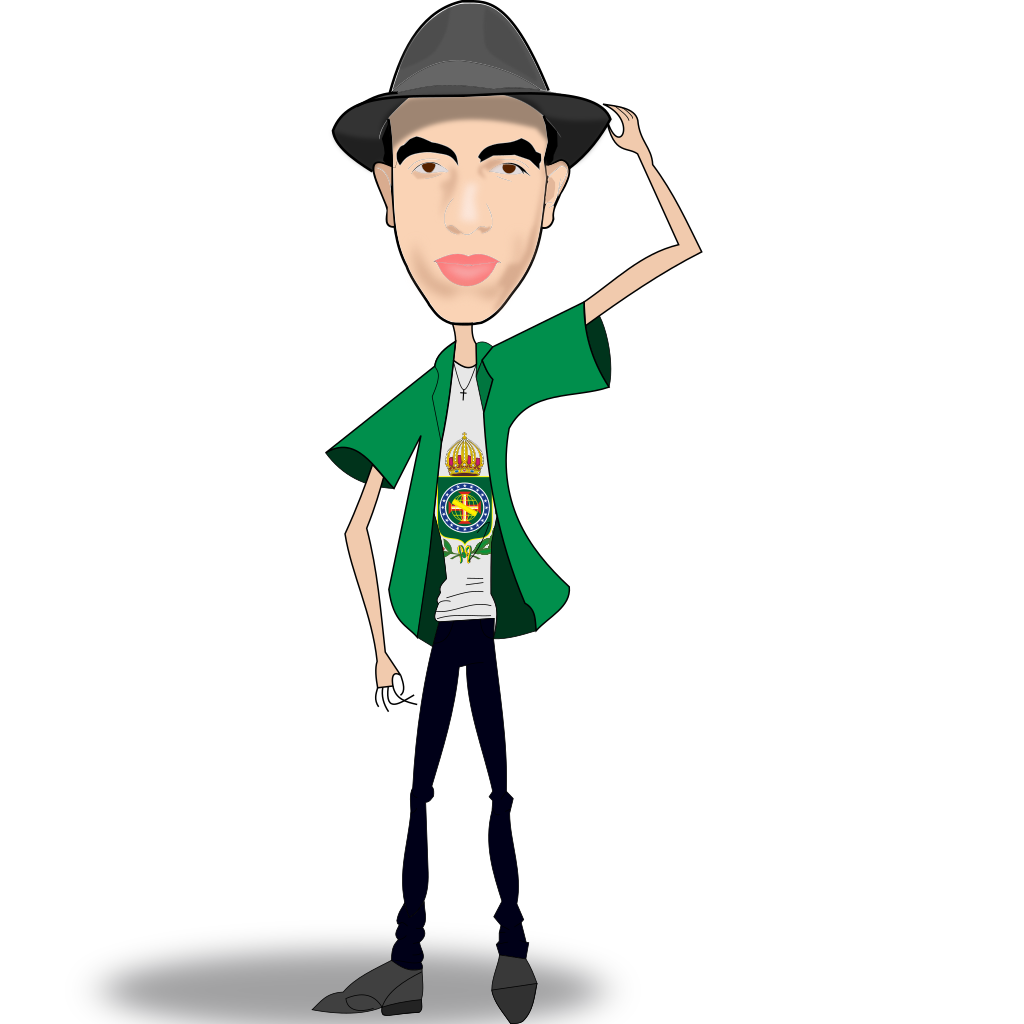
\includegraphics[scale=0.1]{img/NomeDoArquivo}
            \caption{\label{fig:pontos}\footnotesize Numa só.}
         \end{subfigure}

         \legend{\footnotesize Fonte: \url{http://ismaeldamiao.blogspot.com} - Acesso em 20 de nov. 2019.}
      \end{figure}

      Com o \LaTeX  podemos adcionar gráficos:

      \begin{figure}[H]
         \centering
         \caption{\label{fig:hooke}\footnotesize Exemplo de gráfico com GNUPlot.}
         \begin{gnuplot}[terminal=pdf]
            set key box top left
            data = "data/1.dat"

            set ylabel "Força (N)"
            set xlabel "Deslocamento (m)"

            f(x) = A * x + B

            fit f(x) data via A, B

            plot data lc rgb "blue" pt 4 ps .9 title "Dados", \
            f(x) w lp pt 7 ps 0.1 lc rgb "red" title "Ajuste linear"
         \end{gnuplot}
      \end{figure}

      Com o \LaTeX  podemos adcionar estruturas químicas:

      \begin{figure}[H]
         \centering
         \caption{\label{fig:polipropileno}\footnotesize Exemplo de estrutura química ($[C_3H_6]_n$).\cite{polipropileno}}
         \chemfig{
            \vphantom{CH_2}-[@{op,.75}]CH_2-CH(-[6]CH_3)-[@{cl,0.25}]
         }
         \makebraces[5pt,25pt]{\!\!\!n}{op}{cl}
         \bigskip
      \end{figure}

      {\let\clearpage\relax 
   \chapter{Conclusões}
      \vspace{0.5cm}}

      Com base nos dados obtidos concluímos que a lei é verdadeira/falsa. (nessa parte 'venda' seu experimento, é aqui que você mostra o que sabe)

% ------------------------------------------------------------------------------
% ELEMENTOS PÓS-TEXTUAIS
% ------------------------------------------------------------------------------
   \postextual

   {\let\clearpage\relax 
   \chapter{Apêndice}}

      \noindent Grau de precisão:

      Para este experimento desconsideraram-se fatores como a resistência do ar, o pouco atrito e a má distribuição das forças 
      sobre os corpos extensos, assim assumimos um grau de precisão de até $5\%$. \\

      \noindent Variação percentual:

      Neste relatório, todos as diferenças percentuais $Er_\%$ entre dois valores quaisquer $\varphi_e$ e $\varphi_t$, com 
      $\varphi_e\geq\varphi_t$, foram 
      calculadas da seguinte forma:

      \begin{equation} \label{eq:errper}
         Er_\% = \frac{\varphi_e - \varphi_t}{\varphi_t}100\%
      \end{equation}

      \noindent Incerteza:

      Neste relatório, a média $\overline{\varphi}$ dos $n$ valores $\varphi$ em um conjunto de dados qualquer possui uma 
      incerteza associada $\Delta \overline{\varphi}$ da forma:

      \begin{equation}\label{eq:incet}
         \Delta \overline{\varphi} = ± \sum_{i=1}^{n} \frac{| \varphi_i - \overline{\varphi}|}{n}
      \end{equation}

   % ---------------------------------------------------------------------------
   % Referências bibliográficas
   % ---------------------------------------------------------------------------
   \bibliography{reference}

\end{document}
